\section{Architecture}
This section describes the internal architecture of Spring XD. See
figure~\ref{fig:architecture}.

\subsection{Application Context}
The foundation of Spring XD is the Spring application context. The application
context is a dependency injection framework that is used to instantiate
objects along with their dependencies \cite{spring-framework-reference}.
The application context provides a consistent means of declaring dependencies
and configuration for applications written in Java. All projects in the
Spring portfolio depend on the application context.

\subsection{Modules}
A Spring XD Module is a unit of data processing. A stream processing module
for Spring XD consists of one of three types: sources, processors, and sinks.
A stream consists of a collection of modules that define a pipeline for data. 
Job modules are responsible for the execution of batch jobs.

Modules in Spring XD are defined in their own application context. This allows
for easy encapsulation and life cycle management for modules. Additionally,
the use of an application context allows for easy module expansion.

\subsection{Message Bus}
Modules require a data transport in order to transfer data. Spring XD
supports pluggable transports via a messaging abstraction known as 
the Message Bus. Spring XD includes implementations based on Redis, RabbitMQ,
and Kafka. Each of the message bus implementations are provided by the
Spring Integration project.

\subsection{Containers}
A Spring XD container consists of a JVM running an application context which
load child application contexts for modules on demand. Depending on the modules
being executed by the container, the container will also create connections to
the message bus. The capacity of a Spring XD system can be expanded by running
multiple containers.

\subsection{Admin}
The Spring XD admin server hosts a REST service used for Spring XD
administration and the orchestration of streams and jobs. While a single
admin server is required, multiple admin servers may be present in a Spring XD
system for redundancy. A single admin server will be responsible for stream
and job deployments. If multiple admin servers are present, a "supervisor"
server will be selected 

\subsection{ZooKeeper}
Apache ZooKeeper is a distributed configuration and synchronization service.
It provides primitives required for coordination of distributed systems.
In the case of Spring XD, ZooKeeper is used for: \begin{itemize*}
	\item Centralized storage for streams and jobs
	\item Tracking of containers and the modules they are hosting
	\item Notification of arriving and departing containers
	\item Notification of stream/job deployments and un-deployments
\end{itemize*}
\begin{figure}[ht]
\centering
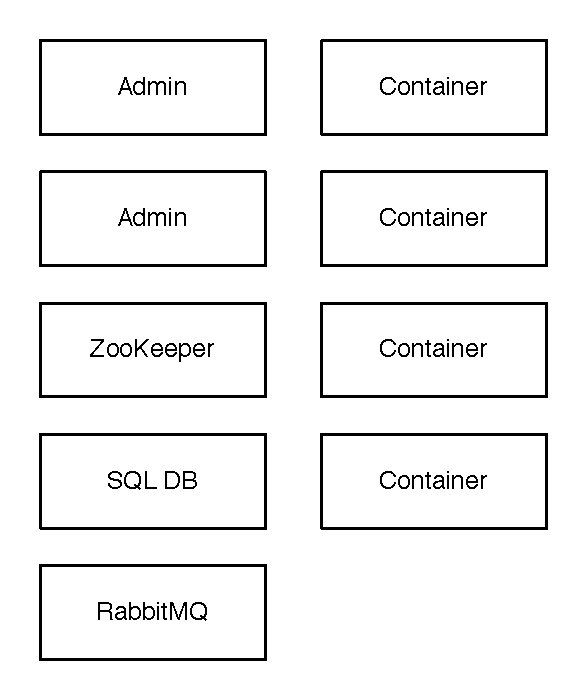
\epsfig{file=XD-sample.eps, height=2in, width=2in}
\caption{Spring XD Architecture.}
\label{fig:architecture}
\end{figure}

